\section{Evaluation}
\label{sec:evaluation}
% We evaluate \OurSys using different types of traffic to measure its improvement
% to application-level behavior in the presence of lossy links.

We evaluated \OurSys with microbenchmarks and network simulation.
% to answer these questions:
%\begin{itemize}

%\item What are the resource requirements for \OurSys with different levels of 
%error correction?

%\item How much does \OurSys improve application throughput across lossy links?

%\item What benefit can \OurSys have to networks at large?
%\end{itemize}



% We
% evaluate three possible deployment models for \OurSys: an FPGA external to
% the switch; a software implementation running on the switch CPU; and an ASIC  
% implementation integrated into the switch forwarding engine. 

\subsection{\OurSys models}

\subsubsection{Line Rate P4 Model.} 

% \subsection{Setup}
% \begin{figure}
%   \centering
%   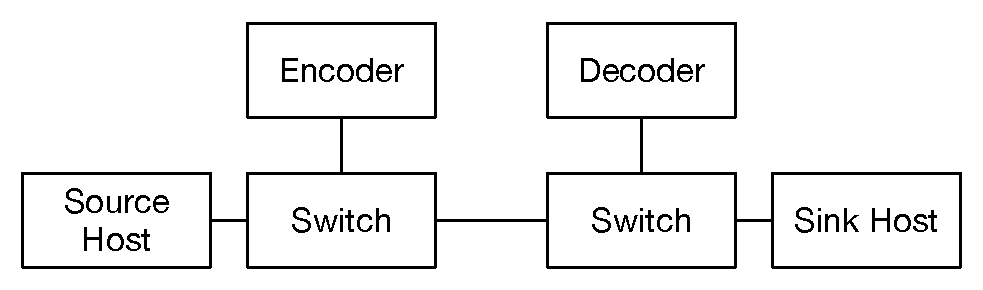
\includegraphics[width=0.3\paperwidth]{exp_topo.pdf}
%   \caption{\label{fig:exp_topo} Testbed topology for benchmarks.}
% \end{figure}

% Figure~\ref{fig:exp_topo} depicts the testbed we used to benchmark \OurSys.
% \hg{This setup was not used to test the FPGA, so it probably does not
% belong in a section on its own.}
% The two traffic generation hosts are each connected to different \OurSys
% enabled switches, which are themselves connected by a 10 GbE link. The
% switches are Wedge BF32-100X's with Barefoot Tofino~\cite{tofino} P4 
% programmable forwarding engines. \lei{TODO: fix cite}


\begin{figure}
  \centering
  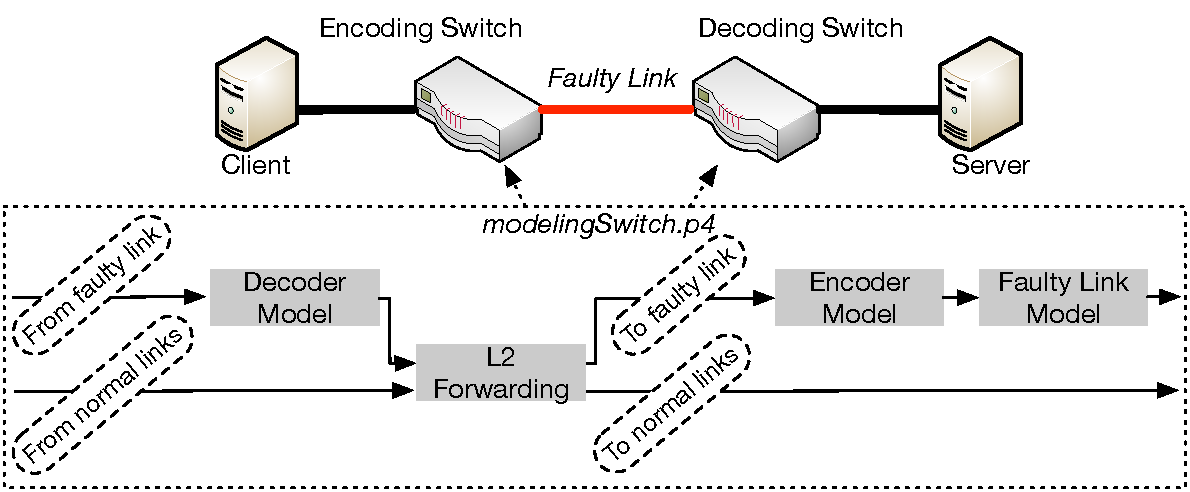
\includegraphics[width=0.4\paperwidth]{figures/lineRateModel.pdf}
  \caption{\label{fig:p4ModelTopo} Topology of the 10 Gb/s testbed 
  network for TCP benchmarks, with line-rate P4 modeling of FEC functionality and faulty links.}
\end{figure}

To measure the effect of faulty links and \OurSys at the application level, we
developed a P4 pipeline for the Barefoot Tofino that models \OurSys. We
deployed the model in a simple 10 Gb/s testbed network, as depicted in
Figure~\ref{fig:p4ModelTopo}, and benchmarked the performance of 
Iperf in real-time. The P4 pipeline models the behavior of the encoder, 
decoder, and faulty link, and can be reconfigured with different FEC and 
packet loss parameters at runtime via the control plane. 

The \textbf{\em encoder model} of the pipeline encapsulates each packet egressing on
the faulty link with the \OurSys header and inserts blank  parity packets into
the flow. It tracks per-port block IDs and  packet indices using P4 register
arrays. To generate parity packets, the  model clones the last data packet in
each block with the Tofino's multicast engine.

The \textbf{\em faulty link model} adds a \emph{corruption header} to each packet
egressing the faulty link. The header indicates whether or not the neighbor
switch should consider the packet lost. The model selects packets for
corruption according to a simple binomial distribution implemented with the
Tofino's random number generator.

Finally, the \textbf{\em decoder model} applies to all packets arriving from a
faulty link, before any other forwarding logic. It removes the corruption
header from each packet and passes non-corrupt packets to the forwarding
pipeline. The model recirculates corrupt packets until the next block begins,
at which point it decides whether they can be recovered based on the number of
non- corrupt data and parity packets it has observed in the block. If it
counted at least K data plus parity packets  in the block, the model
"recovers" all of the corrupt packets by simply removing their corruption
headers and forwarding them normally. If recovery fails, the model drops the
corrupt packets without forwarding.

All experiments we describe below measure performance of 10 second file
transfers from the client to the server, through an encoding switch, faulty
link, and decoding switch. We ran 25 trials for each tested configuration of
K, H,  and loss rate.


\begin{figure*}[!ht]
\centering
\begin{minipage}[b]{0.32\linewidth}
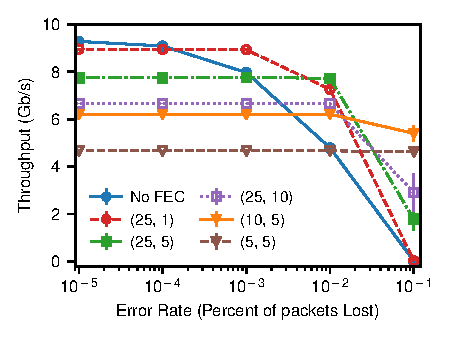
\includegraphics[width=\linewidth]{figures/lossVsTput.pdf}
\caption{Iperf throughput.}
\label{fig:lossVsTput}
\end{minipage}
\hspace{.05in}
\begin{minipage}[b]{0.32\linewidth}
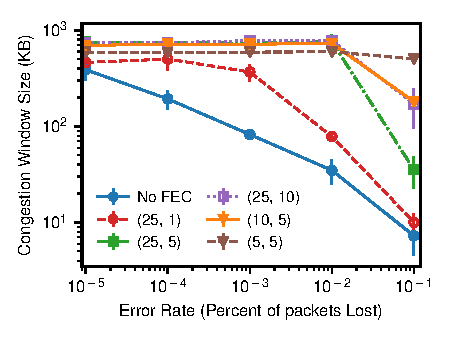
\includegraphics[width=\textwidth]{figures/lossVsWindow.pdf}
\caption{Iperf TCP window sizes.}
\label{fig:lossVsWindow}
\end{minipage}
\hspace{.05in}
\begin{minipage}[b]{0.32\linewidth}
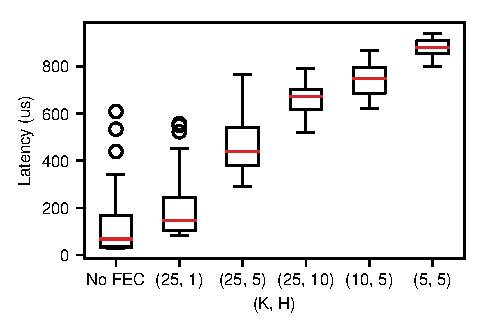
\includegraphics[width=\textwidth]{figures/latency.pdf}
\caption{Network latency.}
\label{fig:latency}
\end{minipage}
\end{figure*}

% \begin{figure}
%   \centering
%   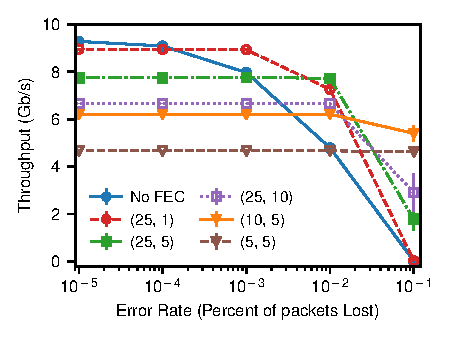
\includegraphics[width=0.3\paperwidth]{figures/lossVsTput.pdf}
%   \caption{\label{fig:lossVsTput} Iperf throughput at different loss rates.}
% \end{figure}

% \begin{figure}
%   \centering
%   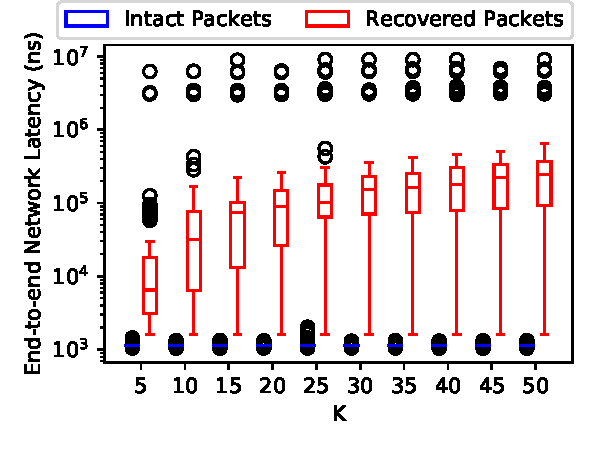
\includegraphics[width=0.3\paperwidth]{figures/udpLatency.pdf}
%   \caption{\label{fig:lossVsLatencyUdp} Network latency for a 100 Mb/s UDP flow (H = 5, loss rate = $10 ^{-2}$).}
% \end{figure}

% \begin{figure}
%   \centering
%   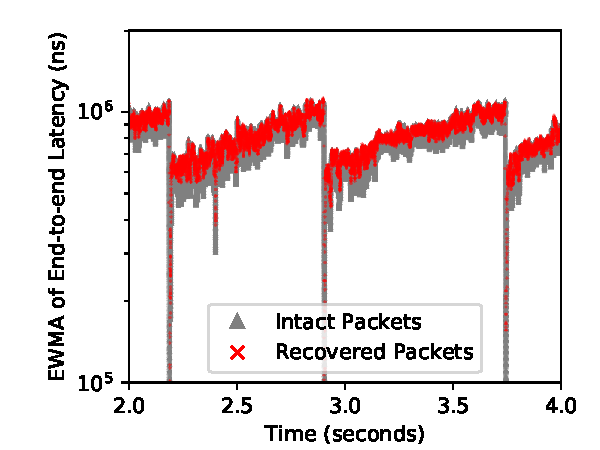
\includegraphics[width=0.3\paperwidth]{figures/tcpLatency.pdf}
%   \caption{\label{fig:lossVsLatencyTcp} Network latency for a 9 Gb/s TCP flow (K = 25, H = 5, loss rate = $10 ^{-2}$).}
% \end{figure}

Figure~\ref{fig:lossVsTput} shows TCP throughput with different FEC
configurations as loss rate varied. With \OurSys, Iperf sustained  over 5 Gb/s
with loss up to $10^{-1}$ (1 out of every 10 packets dropped). Without
\OurSys, Iperf's throughput at that loss rate was under 25 Mb/s. 

Figure~\ref{fig:lossVsWindow} shows average congestion window sizes in 
the trials. Congestion window size ($cwnd$) determines how much data the sender 
can transmit before receiving an ACK, limiting the transmission rate 
to approximately $cwnd$ * round trip time. TCP increases $cwnd$ linearly 
with successful packet deliveries, and reduces it exponentially upon 
packet loss. As Figure~\ref{fig:lossVsWindow} shows, random packet loss 
at rates higher than around $10^{-5}$ causes TCP to reduce $cwnd$ significantly, 
causing the throughput drop in Figure~\ref{fig:lossVsTput}. With FEC, 
the congestion window remains high as loss rate increases, especially when 
using high levels of redundancy, e.g., $(K, H) = (5, 5)$. 

Figure~\ref{fig:latency} shows the in-network latency, i.e., from the  ingress
pipeline of the encoding switch to the egress pipeline of the  decoding
switch, in trials with 0 loss. FEC added under 1 MS of average latency in  all
trials. The amount of latency added by FEC was proportional to $H/K$,  because
the parity packets increased the average length of the egress queue to the
faulty port  by a factor of approximately $H/K$. The additional latency  also
explains why $cwnd$ in Figure~\ref{fig:lossVsWindow} increased with ($H/K$),
as higher latencies require larger window sizes to reach optimal throughput.
\lei{\#Shrink Candidate\#}




% % This figure shows the impact of H. 

% Figure~\ref{fig:lossVsTput} also shows the bandwidth overhead of  FEC, which
% is dominated by the number of parity packets per block ($H$).  At loss rates
% greater than or equal to $10^{-4}$ the bandwidth overhead of adding  parity
% packets had less of an impact on TCP throughput than lost packets, for  most
% configurations tested. To reduce bandwidth overhead, the FEC  can be tuned for the
% loss rate of each specific link, which is reportedly stable over
% time~\cite{corropt}.



% % This figure shows the impact of K.

% To understand how FEC impacts latency, we measured the latency  between the
% ingress pipeline from the source server and the egress pipeline  to the sink
% server, using the nanosecond precision  timestamps of the Tofino, with packets
% routed back through the first  switch before egressing to the sink.
% Figure~\ref{fig:lossVsLatencyUdp}  plots an EWMA of latency for packets in a
% 100 Mb/s UDP flow. For  intact packets, latency was low because they did not
% invoke  the decoder. For  recovered packets, however, the decoder increased
% latency. Average  latency increased with block size because  recovery requires
% the decoder to wait until all the parity packets  for a block arrive. The
% maximum observed latency for recovered packets  was high, around 9 MS. This
% was due to the behavior of the iperf  UDP generator, which periodically paused
% for up to 9 MS between  sending packets, to meet the 100 Mb/s target. The high
% inter-packet  arrival time stalled the generation of parity packets and thus
% the  recovery of any lost packets in the same block.
% \lei{\#Shrink Candidate\#}

% Figure~\ref{fig:lossVsLatencyTcp} plots a time series of latency EWMA  for TCP
% packets in a single maximum rate flow (around 9 Gb/s). The difference in
% latency between recovered versus intact packets was almost indistinguishable.
% Latency for all packets was not dominated by the decoder, but instead by time
% spent  in egress buffers in the switch, which repeatedly filled due to TCPs
% congestion  control dynamics, i.e., causing the familiar ``sawtooth'' pattern
% in Figure~\ref{fig:lossVsLatencyTcp}. Additionally, the latency for packet
% recovery was lower with the TCP workload because average packet rate was
% around 1 order of magnitude higher.







\subsubsection{Event-based simulation}
We customised a fat-tree datacenter topology in ns-3~\cite{ns3-dcn} to
model (i)~a link with loss characteristics as described by Zhuo et
al.~\cite{Zhuo:2017:UMP:3098822.3098849}; and (ii)~FEC to support
transport protocols. In this model we experimented with end-to-end
error correction rather than link-layer, to simulate a more complex
implementation without incurring the burden of implementing it fully.

Table~\ref{tab:ns3} shows our results for a simulation of a 128-node
fat-tree network with 10Gbps links where two nodes communicate over
TCP. We see that end-to-end FEC incurs significant end-to-end
overhead, making it less appealing than the link-layer design we opted
for in this paper.

\begin{table}
% \footnotesize
\begin{center}
\small
\begin{tabular}{c|cc|c}
\toprule
 & \multicolumn{2}{|c|}{Retransmitted packets} & \\
Link loss & no FEC & FEC & FEC Overhead (\%) \\
\midrule
$10^{-3}$ & 152  & 0 & 20 \\
$10^{-4}$ & 23   & 0 & 20 \\
$10^{-5}$ & 2    & 0 & 20 \\
\bottomrule
\end{tabular}
\caption{TCP retransmission behaviour with FEC, and FEC's overhead.
  We model sending 10MB at 2Gbps. For FEC we used a block size of 6,
  consisting of 5 data packets and 1 parity packet.
}
\label{tab:ns3}
\end{center}
\end{table}


\subsection{Encoder Microbenchmarks}
\iffalse
Here we evaluate the implementation directly, not using a model.
Latency and throughput graphs for experiments involving different loss rates, and the encoder working on the CPU and FPGA.
Note: we have not optimized the CPU implementation.
\fi
We measured the performance of our current encoder implementation, which has a
few restrictions.  The encoder parameters are fixed to $k = 8$ and $h = 4$,
and it handles only a single flow of packets with 1024-byte payloads.
Packets were supplied to the FPGA with the packet generator of DPDK 17.08.1.
At the output, we measured a throughput of 9.025 Gbps over a 10-minute period,
nearly saturating the 10-Gbps link.

\iffalse
To ensure \OurSys's effect observed in the model are practical, we directly measured the 
full throughput of our encoder implementation in FPGA. For our benchmark, the encoder is configured to use
k=8 and h=4. Packets are generated by a tool based
on DPDK library, and are fed to the board (as is specified above~(\S\ref{sec:implementation})) through
a 10Gbps link. The average outgoing throughput measured during a 10 minutes test is 9.025Gbps.
Considering the overhead from other parts of the system, we believe the link is actually close
to being saturated, which is our basic assumption in evaluations.
\fi

As a contrast, we also evaluated the CPU implementation (not optimized). Under the same deployment, the throughput measured is 
(\$CPUVALUE), (\$RATIO) lower compared to FPGA.
\lei{TODO: fill the number} \lei{\#Shrink Candidate\#}


\subsection{FPGA resource consumption}
Table~\ref{tab:microbenchmarks} shows the resource requirements for the FPGA implementations of
\OurSys with different $k$ and $h$ parameters.  The resource requirements are
post-implementation utilization values reported by Xilinx Vivado.  We observe
that varying $k$ has a negligible effect on resource consumption, whereas BRAM
consumption has a strong dependence on $h$.  We believe that the BRAM consumption
can be further reduced because several arrays were overpartitioned.
%CPU cycles for the software
%implementation are measured using Linux performance counters and averaged over
%X packets,
The timing statistics are measured using ingress and egress timestamps on
the switch.

\iffalse
\begin{table}
% \footnotesize
\begin{center}
\small
% \resizebox{\linewidth}{!}{
\begin{tabular}{ l l l l l l l } 
\toprule
$(k, h)$ & $(25, 1)$ & $(25, 5)$ & $(25,10)$ & $(50, 1)$ & $(50, 5)$ & $(50, 10)$ \\
\midrule
\emph{Software} & & & & & & \\
\cmidrule{1-1}
Cycles & & & & & & \\
Proc. Time (ns) & & & & & & \\
\midrule
\emph{FPGA} & & & & & & \\
\cmidrule{1-1}
BRAM (18Kb) & 135 (7\%) & 186 (10\%) & 248 (14\%) & 135 (7\%) & 186 (10\%) & 248 (14\%) \\
DSP & 0 (0\%) & 0 (0\%) & 0 (0\%) & 0 (0\%) & 0 (0\%) & 0 (0\%) \\
Flip-flop & 52420 (10\%) & 53415 (10\%) & 54497 (10\%) & 52420 (10\%) & 53416 (10\%) & 54496 (10\%) \\
LUT & 31372 (11\%) & 32439 (12\%) & 33136 (12\%) & 31368 (11\%) & 32479 (12\%) & 33215 (12\%) \\
Proc. Time (ns) & & & & & & \\
\bottomrule
\end{tabular}
% }
\caption{Resource requirements for FPGA and CPU implementations of \OurSys with different configurations.}
\label{tab:microbenchmarks}
\end{center}
\end{table}
\fi

\begin{table}
% \footnotesize
\begin{center}
\small
% \resizebox{\linewidth}{!}{
\begin{tabular}{ l r r r r } 
\toprule
$(k, h)$ & $(25, 1)$ & $(25, 5)$ & $(25,10)$ & $(50, 1)$ \\
\midrule
\emph{Software} & & & & \\
\cmidrule{1-1}
Cycles & & & & \\
Proc. Time (ns) & & & & \\
\midrule
\emph{FPGA} & & & & \\
\cmidrule{1-1}
BRAM (18Kb) & 135 (7\%) & 186 (10\%) & 248 (14\%) & 135 (7\%) \\
DSP & 0 (0\%) & 0 (0\%) & 0 (0\%) & 0 (0\%) \\
Flip-flop & 52420 (10\%) & 53415 (10\%) & 54497 (10\%) & 52420 (10\%) \\
LUT & 31372 (11\%) & 32439 (12\%) & 33136 (12\%) & 31368 (11\%) \\
Proc. Time (ns) & & & & \\
\bottomrule
\end{tabular}
% }
\caption{Resource and Performance Comparison of FPGA and CPU implementations of \OurSys with different configurations.}
\label{tab:microbenchmarks}
\end{center}
\end{table}

%We run \OurSys in 3 configurations: outside the switch, on the switch, and in the switch.
%Time how quickly \OurSys reacts to failing links.
